\chapter{Greedy Algorithms}

In the previous chapter you learned to be patient. Dynamic programming
never commits to a choice until it has
considered all the alternatives, stored their answers in a table, and compared
them. It is thorough, careful, and a little slow. This
chapter takes the opposite approach. A \emph{greedy} algorithm is
impatient. At every step it grabs the choice that looks best \emph{right now},
locks it in permanently, and moves on without building a table of alternatives.

For certain problems this purely local strategy produces a provably
\emph{optimal} global solution -- matching what an exhaustive dynamic program
would find, in a fraction of the time and memory. The central challenge of this
chapter is telling \emph{when} a greedy rule is provably optimal and when it
fails, because a plausible greedy heuristic is also one of the easiest ways to
write an algorithm that is fast, simple, and wrong on subtle inputs.

We solve a scheduling problem twice --
once the greedy way and once the dynamic-programming way -- and watch them
agree, then distill the two structural properties every greedy proof leans
on. From there we build Huffman's optimal compression code from scratch, byte by byte.
The chapter closes with \emph{matroids}, the abstraction that
explains, in one theorem, an entire family of problems where greed is
guaranteed to win.

\chapterline

\section{A first taste: choosing activities}

Start with a concrete scheduling problem. You have a single shared
resource -- a lecture hall, a tennis court, a telescope -- and a pile of
requests to use it. Each request is an \emph{activity} with a fixed start time
and a fixed finish time. Two activities are \emph{compatible} if they do not
overlap in time; you cannot run two things in the hall at once. Your goal is to
schedule as \emph{many} activities as possible.

That last word matters: you are maximizing the \emph{count} of activities, not
the total time used, not anyone's preference. Just the number of non-overlapping
talks you can squeeze in.

Here is a concrete set. We give each activity an index $i$, a start $s_i$,
and a finish $f_i$, and -- this will matter shortly -- we have sorted them by
\emph{finish time}.

\begin{center}
\begin{tabular}{c|ccccccccccc}
\toprule
$i$   & 1 & 2 & 3 & 4 & 5 & 6 & 7 & 8 & 9 & 10 & 11 \\
$s_i$ & 1 & 3 & 0 & 5 & 3 & 5 & 6 & 8 & 8 & 2  & 12 \\
$f_i$ & 4 & 5 & 6 & 7 & 9 & 9 & 10 & 11 & 12 & 14 & 16 \\
\bottomrule
\end{tabular}
\end{center}

This is the exact instance CLRS uses, and it is worth keeping on a sticky note.
Activity 1 runs during the time interval $[1,4)$, activity 2 during $[3,5)$, and
so on. Activities 1 and 2 overlap (both want the room around time $3.5$), so they
are \emph{not} compatible. Activities 1 and 4 do not overlap ($[1,4)$ and
$[5,7)$), so they are.

\begin{intuitionbox}
Picture the day as a long horizontal timeline and each activity as a horizontal
bar laid across it from its start to its finish. ``Compatible'' just means
``these two bars do not touch.'' You want to lay down as many bars as you can
without any two overlapping. Stack them on a single shelf; how many fit?
\end{intuitionbox}

\begin{figure}[h]
\centering
\begin{tikzpicture}[xscale=0.62,yscale=0.5]
  % axis
  \draw[->] (0,0) -- (17,0) node[right]{time};
  \foreach \x in {0,2,4,6,8,10,12,14,16}
    \draw (\x,0.1) -- (\x,-0.1) node[below,font=\scriptsize]{\x};
  % bars: each at a row, drawn from s to f
  \newcommand{\act}[5]{\draw[fill=#4] (#2,#1-0.18) rectangle (#3,#1+0.18);
    \node[font=\scriptsize] at (#2-0.0,#1+0.55) {$a_{#5}$};}
  \act{1}{1}{4}{green!25}{1}
  \act{2}{3}{5}{red!15}{2}
  \act{3}{0}{6}{red!15}{3}
  \act{4}{5}{7}{green!25}{4}
  \act{5}{3}{9}{red!15}{5}
  \act{6}{5}{9}{red!15}{6}
  \act{7}{6}{10}{red!15}{7}
  \act{8}{8}{11}{green!25}{8}
  \act{9}{8}{12}{red!15}{9}
  \act{10}{2}{14}{red!15}{10}
  \act{11}{12}{16}{green!25}{11}
\end{tikzpicture}
\caption{The eleven activities as bars. Highlighted in green is one optimal
selection $\{a_1, a_4, a_8, a_{11}\}$ of four mutually non-overlapping
activities. No selection of five exists.}
\label{ch16:activity-bars}
\end{figure}

\subsection{The greedy guess}

Faced with this, your instinct might be to try several rules of thumb. ``Pick
the shortest activity first, to leave room for others.'' ``Pick the activity that
overlaps the fewest others.'' ``Pick the one that starts earliest.'' Some of
these sound reasonable. Most of them are \emph{wrong} -- we will break them in a
moment. But one rule, almost suspiciously simple, is provably right:

\begin{focusbox}
\textbf{The greedy rule for activity selection.} Among all activities still
compatible with what you have chosen, always pick the one that \emph{finishes
earliest}. Then throw away everything that conflicts with it and repeat.
\end{focusbox}

Why finish-earliest? Because finishing early is exactly the property that leaves
\emph{the most room} for everything that comes after. When you commit to the
activity with the smallest finish time, you free up the resource as soon as
possible, maximizing the remaining open timeline for future choices. The rest of
this section makes this precise.

Because we sorted by finish time, the greedy rule becomes almost trivial to
execute: scan left to right, and grab an activity whenever it does not collide
with the last one you grabbed.

\begin{labbox}
Let us trace it on the table. We pick $a_1$ (finish $4$) -- it is first, so take
it. Now scan for the next activity whose \emph{start} is $\ge 4$. Activity $2$
starts at $3$: too early, skip. Activity $3$ starts at $0$: skip. Activity $4$
starts at $5 \ge 4$: \textbf{take it}. Last finish is now $7$. Scan on: $a_5$
starts $3$, $a_6$ starts $5$, $a_7$ starts $6$ -- all $< 7$, skip. $a_8$ starts
$8 \ge 7$: \textbf{take it}. Last finish $11$. $a_9$ starts $8$, $a_{10}$ starts
$2$ -- skip. $a_{11}$ starts $12 \ge 11$: \textbf{take it}. We end with
$\{a_1, a_4, a_8, a_{11}\}$ -- four activities. Go back to
Figure~\ref{ch16:activity-bars} and confirm the green bars never touch.
\end{labbox}

\subsection{The algorithm}

Here is the routine. We assume the activities arrive already sorted so that
$f_1 \le f_2 \le \cdots \le f_n$; if they are not, sorting first costs an extra
$O(n \log n)$, which we will fold into the analysis.

\begin{algorithm}[H]
\caption{\textsc{Greedy-Activity-Selector}($s, f, n$)}
\KwIn{Start times $s[1\mathinner{\ldotp\ldotp} n]$ and finish times $f[1\mathinner{\ldotp\ldotp} n]$, with $f$ nondecreasing.}
\KwOut{A maximum-size set $A$ of mutually compatible activities.}
$A \leftarrow \{a_1\}$ \tcp*{the first to finish is always safe to take}
$k \leftarrow 1$ \tcp*{$k$ = index of the last activity we added}
\For{$m \leftarrow 2$ \KwTo $n$}{
  \If{$s[m] \ge f[k]$}{
    $A \leftarrow A \cup \{a_m\}$ \tcp*{$a_m$ starts after $a_k$ finishes}
    $k \leftarrow m$ \tcp*{$a_m$ is now the most recent}
  }
}
\Return $A$
\end{algorithm}

The loop runs once per activity and does a constant amount of work each time, so
the loop is $\Theta(n)$. The only state it carries between iterations is $k$, the
index of the last chosen activity -- a single integer. That economy of state is a
hallmark of greedy algorithms.

\begin{complexitybox}
If the input is already sorted by finish time, \textsc{Greedy-Activity-Selector}
runs in $\Theta(n)$ time and $\Theta(1)$ extra space (beyond the output). If you
must sort first, the total is $\Theta(n \log n)$, dominated by the sort.
Contrast this with a dynamic-programming solution to the same problem, which
fills an $n \times n$ table in $\Theta(n^3)$ or, carefully, $\Theta(n^2)$ time.
Greed is simpler here and also asymptotically faster.
\end{complexitybox}

\subsection{Why is it correct? The exchange argument}

A fast wrong answer is worthless, so we owe you a proof. The standard tool for
greedy correctness is the \emph{exchange argument}: take any optimal solution,
and show you can edit it -- swap one element for the greedy choice -- without
making it worse. If the greedy choice can always be substituted in, then there is
an optimal solution that \emph{contains} the greedy choice, so greed loses
nothing by taking it.

\begin{theorem}[Greedy is optimal for activity selection]
\label{ch16:thm-activity}
Let $a_1$ be the activity with the earliest finish time. Then some maximum-size
set of mutually compatible activities includes $a_1$.
\end{theorem}

\begin{formalbox}
\textbf{Proof.} Let $A$ be any maximum-size compatible set, and let $a_j$ be the
activity in $A$ with the earliest finish time. If $a_j = a_1$ we are done.
Otherwise, form $A' = (A \setminus \{a_j\}) \cup \{a_1\}$: throw out $a_j$, throw in
$a_1$. We claim $A'$ is still a valid set of the same size.

Same size: we removed one activity and added one, so $|A'| = |A|$.

Still compatible: every activity in $A$ other than $a_j$ starts no earlier than
$a_j$ finishes (since $a_j$ finishes earliest in $A$ and they are all pairwise
compatible). But $a_1$ finishes \emph{no later} than $a_j$, because $a_1$ has the
globally earliest finish time, i.e. $f_1 \le f_j$. So everything that did not
conflict with $a_j$ cannot conflict with $a_1$ either -- $a_1$ vacates the room
even sooner. Hence $A'$ is compatible.

So $A'$ is a maximum-size compatible set containing $a_1$. $\qquad\blacksquare$
\end{formalbox}

Figure~\ref{ch16:fig-exchange-argument} illustrates this substitution: because $a_1$ finishes at or before $a_j$ ($f_1 \le f_j$), swapping $a_1$ in place of $a_j$ vacates the room even earlier, leaving every subsequent activity in $A$ completely conflict-free.

\begin{figure}[h]
\centering
\begin{tikzpicture}[font=\small]
  % Top track: Optimal solution A
  \node[font=\footnotesize\bfseries, text=quotientorange!90!black, left] at (0.8, 2.0) {Optimal $A$:};
  
  % a_j in A
  \draw[thick, draw=quotientorange, fill=quotientorange!20, rounded corners=1.5pt] (1.8, 1.7) rectangle (5.2, 2.3);
  \node[font=\scriptsize\bfseries, quotientorange!90!black] at (3.5, 2.0) {earliest in $A$: $a_j$};

  % Other activities in A
  \draw[thick, draw=gray!60, fill=gray!12, rounded corners=1.5pt] (5.8, 1.7) rectangle (8.4, 2.3);
  \node[font=\scriptsize, text=gray!80!black] at (7.1, 2.0) {$a_k \in A$};
  
  \draw[thick, draw=gray!60, fill=gray!12, rounded corners=1.5pt] (9.0, 1.7) rectangle (12.0, 2.3);
  \node[font=\scriptsize, text=gray!80!black] at (10.5, 2.0) {$a_m \in A$};

  % Bottom track: Exchanged solution A'
  \node[font=\footnotesize\bfseries, text=targetgreen!90!black, left] at (0.8, 0.5) {Exchanged $A'$:};
  
  % a_1 in A'
  \draw[very thick, draw=targetgreen, fill=targetgreen!25, rounded corners=1.5pt] (1.0, 0.2) rectangle (3.8, 0.8);
  \node[font=\scriptsize\bfseries, targetgreen!80!black] at (2.4, 0.5) {greedy choice: $a_1$};

  % Other activities in A' (identical)
  \draw[thick, draw=gray!60, fill=gray!12, rounded corners=1.5pt] (5.8, 0.2) rectangle (8.4, 0.8);
  \node[font=\scriptsize, text=gray!80!black] at (7.1, 0.5) {$a_k \in A'$};
  
  \draw[thick, draw=gray!60, fill=gray!12, rounded corners=1.5pt] (9.0, 0.2) rectangle (12.0, 0.8);
  \node[font=\scriptsize, text=gray!80!black] at (10.5, 0.5) {$a_m \in A'$};

  % Vertical markers and finish time comparison
  \draw[dotted, thick, quotientorange] (5.2, 2.5) -- (5.2, 0.0) node[below, font=\tiny, text=quotientorange!90!black] {$f_j$};
  \draw[dotted, thick, targetgreen] (3.8, 2.5) -- (3.8, 0.0) node[below, font=\tiny, text=targetgreen!80!black] {$f_1$};

  % Exchange arrow
  \draw[-{Latex[length=2.2mm]}, thick, dashed, trapred] (2.6, 1.6) -- 
    node[midway, left=2pt, font=\tiny\bfseries, text=trapred] {swap} (2.1, 0.9);

  % Finish time clearance arrow
  \draw[{Latex[length=1.5mm]}-{Latex[length=1.5mm]}, thick, gray!70!black] (3.8, 1.25) -- 
    node[midway, above=1pt, font=\tiny, text=gray!70!black] {$f_1 \le f_j$} (5.2, 1.25);

  % Explanation banner
  \node[draw=gray!30, fill=white, rounded corners=2pt, font=\scriptsize, align=center] at (6.5, -0.9) {
    \textbf{Exchange invariant}: since $f_1 \le f_j$, any activity starting after $f_j$ also starts after $f_1$.\\
    Thus $A' = (A \setminus \{a_j\}) \cup \{a_1\}$ is compatible, with $|A'| = |A|$ and contains the greedy choice.
  };
\end{tikzpicture}
\caption{The greedy exchange argument. Given an optimal solution $A$ whose first finishing activity is $a_j$, replacing $a_j$ with the greedy choice $a_1$ preserves compatibility because $f_1 \le f_j$. All subsequent activities in $A$ finish after $f_j \ge f_1$, so $A'$ remains compatible and optimal while containing $a_1$.}
\label{ch16:fig-exchange-argument}
\end{figure}

The theorem handles the \emph{first} choice. What about the rest? Once $a_1$ is
fixed, every remaining activity that conflicts with it is useless, and the
problem shrinks to ``select a maximum set among the activities that start at or
after $f_1$.'' That is a smaller instance of the \emph{exact same problem}. So we
apply the theorem again to the subproblem, and again, and again. This is an
induction: each greedy choice is safe, and what remains is a smaller version of
the original. That structure -- \emph{a greedy choice plus one subproblem} -- is
the skeleton of every argument in this chapter.

\begin{trapbox}
It is tempting to ``prove'' greedy works by checking it on a few examples and
declaring victory. Do not. The danger is that wrong greedy rules
\emph{also} pass small examples. The shortest-first rule, for instance, gives the
right answer on plenty of inputs -- and then quietly fails. Only an exchange
argument or an explicit counterexample settles the question.
\end{trapbox}

\subsection{Breaking the wrong rules}

To see how sensitive greedy correctness is to the exact rule, let us rule out two
plausible alternatives with small counterexamples.

\textbf{Shortest-duration-first.} Consider three activities: $[1,5)$, $[4,6)$,
$[5,9)$. The shortest is $[4,6)$ (length $2$), so a shortest-first greedy grabs
it -- and now \emph{both} other activities conflict with it, so it ends with one
activity. But $[1,5)$ and $[5,9)$ are compatible: the optimal answer is two.
Shortest-first loses.

\textbf{Fewest-conflicts-first.} You can build instances (CLRS Exercise 16.1-3
walks you through one) where always taking the activity that overlaps the fewest
others also fails. The earliest-finish rule is special; near-misses are not good
enough.

\begin{walkbox}
Take a walk and try to \emph{break} the earliest-finish rule. Sketch activities
on a timeline and hunt for a case where finishing earliest leads you astray. You
will not find one -- but the act of failing to find one, and feeling \emph{why}
it always leaves the most room behind, will cement the proof better than reading
it twice.
\end{walkbox}

\section{Greedy versus dynamic programming}

You have now met two paradigms that both solve optimization problems by combining
solutions to subproblems. They look similar on the page. When do you reach for
which? Greedy is really a \emph{special case} of dynamic
programming that you are allowed to use only when the problem is unusually
well-behaved. Let us pin down what ``well-behaved'' means.

Both paradigms require \textbf{optimal substructure}: an optimal solution to the
whole contains optimal solutions to its subproblems. That is shared. The thing
greedy demands \emph{on top} is the \textbf{greedy-choice property}.

\begin{focusbox}
\textbf{Greedy-choice property.} You can assemble a globally optimal solution by
making a \emph{locally} optimal (greedy) choice and then solving the \emph{one}
subproblem that remains. Key point: the greedy choice is made \emph{before} the
subproblem is solved -- it does not depend on the answers to any subproblems.
\end{focusbox}

That last sentence is the key difference. In dynamic programming, the choice at
the top \emph{depends} on having already computed the subproblem answers -- you
compare alternatives and pick the best, which is why you need the table. In a
greedy algorithm, you can decide the top-level move \emph{up front}, with no table
at all, because a simple local rule (``earliest finish'') is guaranteed to be
part of some optimal solution.

\begin{figure}[h]
\centering
\begin{tikzpicture}[font=\small]
  % Top Lane: Greedy single-pass scan along the interval timeline
  \begin{scope}[yshift=5.0cm]
    \node[font=\footnotesize\scshape, text=gray!70!black, anchor=west] at (0, 2.2) {Lane 1: Greedy Activity Selection (Single-Pass Horizon Scan)};
    
    % Timeline axis
    \draw[->, thick, gray!70] (0, 0) -- (12.5, 0) node[right, font=\scriptsize] {time};
    \foreach \t in {0, 2, 4, 6, 8, 10, 12} {
      \draw[gray!60] (\t, 0.08) -- (\t, -0.08) node[below, font=\tiny] {\t};
    }
    
    % Activity a1: [1, 4] SELECTED
    \draw[draw=targetgreen, fill=targetgreen!25, very thick, rounded corners=1.5pt] (1, 1.1) rectangle (4, 1.5);
    \node[targetgreen!90!black, font=\tiny\bfseries] at (2.5, 1.3) {$a_1: [1,4]$};
    \node[targetgreen!80!black, font=\tiny, above=1pt] at (2.5, 1.5) {pick 1};
    
    % Activity a2: [3, 5] REJECTED
    \draw[draw=trapred!70, fill=trapred!15, dashed, rounded corners=1.5pt] (3, 0.6) rectangle (5, 1.0);
    \node[trapred!80!black, font=\tiny] at (4, 0.8) {$a_2: [3,5]$};
    
    % Activity a3: [0, 6] REJECTED
    \draw[draw=trapred!70, fill=trapred!15, dashed, rounded corners=1.5pt] (0, 0.1) rectangle (6, 0.5);
    \node[trapred!80!black, font=\tiny] at (3.0, 0.3) {$a_3: [0,6]$ (clashes $s_3 < f_1$)};
    
    % Activity a4: [5, 7] SELECTED
    \draw[draw=targetgreen, fill=targetgreen!25, very thick, rounded corners=1.5pt] (5, 1.1) rectangle (7, 1.5);
    \node[targetgreen!90!black, font=\tiny\bfseries] at (6, 1.3) {$a_4: [5,7]$};
    \node[targetgreen!80!black, font=\tiny, above=1pt] at (6, 1.5) {pick 2};
    
    % Activity a5: [5, 9] REJECTED
    \draw[draw=trapred!70, fill=trapred!15, dashed, rounded corners=1.5pt] (5, 0.6) rectangle (9, 1.0);
    \node[trapred!80!black, font=\tiny] at (7.0, 0.8) {$a_5: [5,9]$ (clashes $s_5 < f_4$)};
    
    % Activity a6: [8, 11] SELECTED
    \draw[draw=targetgreen, fill=targetgreen!25, very thick, rounded corners=1.5pt] (8, 1.1) rectangle (11, 1.5);
    \node[targetgreen!90!black, font=\tiny\bfseries] at (9.5, 1.3) {$a_6: [8,11]$};
    \node[targetgreen!80!black, font=\tiny, above=1pt] at (9.5, 1.5) {pick 3};
    
    % Finish time markers
    \draw[dotted, targetgreen!80!black, thick] (4, 1.5) -- (4, -0.2) node[below, font=\tiny, text=targetgreen!80!black] {$f_1=4$};
    \draw[dotted, targetgreen!80!black, thick] (7, 1.5) -- (7, -0.2) node[below, font=\tiny, text=targetgreen!80!black] {$f_4=7$};
    \draw[dotted, targetgreen!80!black, thick] (11, 1.5) -- (11, -0.2) node[below, font=\tiny, text=targetgreen!80!black] {$f_6=11$};
  \end{scope}

  % Bottom Lane: Decision Space Comparison: DP Branching Tree vs Greedy Spine
  \begin{scope}[yshift=0cm]
    \node[font=\footnotesize\scshape, text=gray!70!black, anchor=west] at (0, 3.4) {Lane 2: Search Space Topology --- Dynamic Programming vs Greedy Strategy};

    % Left side: DP Subproblem Tree (Branching everywhere)
    \begin{scope}[xshift=2.5cm]
      \node[font=\scriptsize\bfseries, text=sourceblue!80!black] at (0, 2.7) {Dynamic Programming ($O(n^2)$ Subproblems)};
      \node[circle, draw=sourceblue, fill=sourceblue!15, thick, inner sep=1.5pt] (dp0) at (0, 2.0) {\scriptsize $S_{0,7}$};
      \node[rounded corners=2pt, draw=gray!60, fill=gray!8, inner sep=2pt] (dp1) at (-1.9, 1.0) {\tiny $k{=}1{:}\, S_{0,1}{+}S_{1,7}$};
      \node[rounded corners=2pt, draw=gray!60, fill=gray!8, inner sep=2pt] (dp2) at (0, 1.0) {\tiny $k{=}2{:}\, S_{0,2}{+}S_{2,7}$};
      \node[rounded corners=2pt, draw=gray!60, fill=gray!8, inner sep=2pt] (dp3) at (1.9, 1.0) {\tiny $\cdots\; k{=}6$};

      \draw[-{Latex[length=1.5mm]}, gray!60] (dp0) -- (dp1);
      \draw[-{Latex[length=1.5mm]}, gray!60] (dp0) -- (dp2);
      \draw[-{Latex[length=1.5mm]}, gray!60] (dp0) -- (dp3);
      
      \node[font=\tiny, text=gray!70!black] at (0, 0.4) {Tries every split $a_k$, solving both $S_{i,k}$ and $S_{k,j}$};
      \node[font=\tiny, text=gray!70!black] at (0, 0.1) {Cost: $O(n^3)$ table fill or $O(n^2)$ memoization};
    \end{scope}

    % Divider
    \draw[dashed, gray!40, thick] (6.0, 0.0) -- (6.0, 3.0);

    % Right side: Greedy Linear Path (No branching!)
    \begin{scope}[xshift=9.5cm]
      \node[font=\scriptsize\bfseries, text=targetgreen!80!black] at (0, 2.7) {Greedy Strategy ($1$ Subproblem Per Step)};
      \node[circle, draw=targetgreen, fill=targetgreen!25, thick, inner sep=1.5pt] (g0) at (0, 2.0) {\scriptsize $S_0$};
      \node[circle, draw=targetgreen, fill=targetgreen!25, thick, inner sep=1.5pt] (g1) at (0, 1.1) {\scriptsize $S_1$};
      \node[circle, draw=targetgreen, fill=targetgreen!25, thick, inner sep=1.5pt] (g2) at (0, 0.2) {\scriptsize $S_4$};
      \node[circle, draw=targetgreen, fill=targetgreen!25, thick, inner sep=1.5pt] (g3) at (0, -0.7) {\scriptsize $S_6$};

      \draw[-{Latex[length=2mm]}, very thick, targetgreen] (g0) -- node[right, font=\tiny, text=targetgreen!90!black] {pick $a_1$ ($f_1$ min)} (g1);
      \draw[-{Latex[length=2mm]}, very thick, targetgreen] (g1) -- node[right, font=\tiny, text=targetgreen!90!black] {pick $a_4$ ($f_4$ min)} (g2);
      \draw[-{Latex[length=2mm]}, very thick, targetgreen] (g2) -- node[right, font=\tiny, text=targetgreen!90!black] {pick $a_6$ ($f_6$ min)} (g3);

      \node[font=\tiny, text=targetgreen!90!black] at (-2.3, 0.5) {\textbf{Zero branching}:};
      \node[font=\tiny, text=gray!70!black] at (-2.3, 0.2) {Earliest finish rule commits};
      \node[font=\tiny, text=gray!70!black] at (-2.3, -0.1) {up front; $O(n)$ total time.};
    \end{scope}
  \end{scope}
\end{tikzpicture}
\caption{Contrasting the decision structure of Greedy Activity Selection with Dynamic Programming. In Lane 1, sorting activities by finish time allows the greedy choice ($a_1$, then $a_4$, then $a_6$) to sweep left-to-right, eliminating conflicting activities without looking ahead. In Lane 2, whereas a full dynamic program must evaluate choices across a branching web of $O(n^2)$ subproblems $S_{i,j}$, the greedy-choice property collapses the search space into a single linear descent path.}
\label{ch16:fig-greedy-vs-dp-activity}
\end{figure}

\subsection{Two coins, one lesson}

The cleanest way to feel the boundary is the \emph{coin-change} problem. You owe
someone $n$ cents and want to pay with the fewest coins.

With U.S. denominations $\{1, 5, 10, 25\}$, the greedy rule -- ``hand over the
largest coin that fits, repeat'' -- is optimal. To make $30$ cents: a quarter
($25$), then a nickel ($5$). Two coins. You cannot do better.

Now change the coin system to $\{1, 3, 4\}$ and make $6$ cents. Greedy grabs the
$4$, then needs $2$ more, which costs two $1$s: total \emph{three} coins
($4+1+1$). But the optimal answer is $3+3$: \emph{two} coins. Greed failed.
Nothing about the algorithm changed -- only the data did -- and the greedy-choice
property no longer held.

\begin{trapbox}
The coin-change lesson is the most important warning in this chapter: whether
greed is correct depends on the \emph{structure of the input}, not on the shape
of the algorithm. The same greedy code is optimal on $\{1,5,10,25\}$ and wrong on
$\{1,3,4\}$. You must \emph{prove} the greedy-choice property for your specific
problem; you cannot inherit it.
\end{trapbox}

For the bad coin system, dynamic programming saves you. Let $C(n)$ be the fewest
coins to make $n$ cents. Then
\[
  C(n) = \min_{d \in \{1,3,4\},\ d \le n} \bigl(1 + C(n-d)\bigr), \qquad C(0)=0,
\]
which tries \emph{every} first coin and keeps the best. Tracing $\{1,3,4\}$ at $n=6$: $C(6) = \min(1+C(5),
1+C(3), 1+C(2))$. With $C(3)=1$ (one $3$-coin), the middle option gives $1+1=2$.
DP finds the $3+3$ answer that greed missed.

Filling the table from $n=0$ upward makes the rescue concrete. Each cell is one
plus the smallest reachable cell a single coin away, and
Figure~\ref{ch16:coin-dp} shows the row in full.

\begin{figure}[h]
\centering
\begin{tikzpicture}[font=\small]
  \matrix (m) [matrix of nodes, nodes={draw, minimum size=8mm, anchor=center},
    column sep=-\pgflinewidth, row sep=-\pgflinewidth,
    nodes in empty cells]
  {
    $n$    & 0 & 1 & 2 & 3 & 4 & 5 & 6 \\
    $C(n)$ & 0 & 1 & 2 & 1 & 1 & 2 & 2 \\
  };
  % highlight the n=6 cell and the n=3 cell it depends on
  \node[draw=targetgreen, line width=1pt, minimum size=8mm] at (m-2-8) {};
  \node[draw=sourceblue, line width=1pt, minimum size=8mm] at (m-2-5) {};
  \draw[->, sourceblue, thick] (m-1-8.north) to[bend right=40]
    node[above, font=\scriptsize]{$+$ one 3-coin} (m-1-5.north);
\end{tikzpicture}
\caption{The coin-change DP table for the system $\{1,3,4\}$. Cell $C(6)=2$
(green) is reached from $C(3)=1$ (blue) by adding a single $3$-coin, recovering
the $3+3$ solution that greedy never considers.}
\label{ch16:coin-dp}
\end{figure}

\begin{table}[h]
\centering
\begin{tabular}{p{0.46\textwidth} p{0.46\textwidth}}
\toprule
\textbf{Dynamic programming} & \textbf{Greedy} \\
\midrule
Choice depends on subproblem solutions; must compute them first. & Choice is made first, by a local rule, before any subproblem is solved. \\
Considers many choices, keeps the best (a $\min$ or $\max$). & Commits to one choice and never revisits it. \\
Needs a table of size proportional to the subproblems. & Needs $O(1)$ extra state. \\
Always correct when there is optimal substructure. & Correct only when the greedy-choice property \emph{also} holds. \\
\bottomrule
\end{tabular}
\caption{Greedy is DP with the freedom to choose first and never look back -- a
freedom you only earn by proving the greedy-choice property.}
\label{ch16:dp-vs-greedy}
\end{table}

\begin{aestheticbox}
This distinction is not academic. A router deciding which packet to forward
next, an operating system picking which job to run, a cache deciding what to
evict -- these systems make \emph{millions} of decisions per second and cannot
afford to build a DP table each time. They run greedy rules. Knowing when a
greedy rule is provably optimal (and when it is merely a fast heuristic you must
test) is the difference between a system that is correct by design and one that
is correct by luck.
\end{aestheticbox}

\subsection{A recipe for designing greedy algorithms}

CLRS distills the design process into a sequence of steps; here it is in plain
language.

\begin{enumerate}
\item \textbf{Cast the problem as a choice.} Reframe ``find the optimal solution''
  as ``make one choice now, then you are left with a single subproblem to solve.''
\item \textbf{Guess a greedy choice.} Propose a local rule -- earliest finish,
  largest coin, smallest weight -- that seems to make the most progress.
\item \textbf{Prove the greedy-choice property.} Show, usually by an exchange
  argument, that there is an optimal solution containing your greedy choice.
\item \textbf{Prove optimal substructure.} Show that after the greedy choice, an
  optimal solution to the rest combines with the choice to give a global optimum.
\item \textbf{Stitch it together by induction.} Greedy choice plus optimal
  subproblem, repeated, yields a global optimum.
\end{enumerate}

Most of the work is in steps 3 and 4. Skip them and you
have a fast algorithm of unknown correctness.

\section{Huffman codes: compression by greed}

Huffman coding is a greedy algorithm you have used
today without knowing it -- it sits inside ZIP, JPEG, MP3, PNG, and the deflate
format used throughout the web. It answers a simple question: given how
often each symbol appears in a file, what is the \emph{shortest} possible way to
encode it?

\subsection{Why variable-length codes}

Suppose a file uses only six characters, $a$ through $f$, with these frequencies
(in thousands of occurrences):

\begin{center}
\begin{tabular}{c|cccccc}
\toprule
character & $a$ & $b$ & $c$ & $d$ & $e$ & $f$ \\
frequency (thousands) & 45 & 13 & 12 & 16 & 9 & 5 \\
\bottomrule
\end{tabular}
\end{center}

A \emph{fixed-length} code gives every character the same number of bits. With
six characters you need $3$ bits each ($2^3 = 8 \ge 6$). Total cost: $(45 + 13 +
12 + 16 + 9 + 5) \times 3 = 100{,}000 \times 3 = 300{,}000$ bits.

But that is wasteful. The character $a$ appears nine times as often as $f$, yet
both get three bits. Surely $a$ deserves a \emph{shorter} codeword and $f$ can
afford a longer one. This is the idea of a \emph{variable-length} code: frequent
symbols get short codes, rare symbols get long ones. The catch is that the
decoder, reading a stream of bits with no separators, must never get confused
about where one codeword ends and the next begins.

\begin{focusbox}
\textbf{Prefix-free codes.} A code is \emph{prefix-free} (CLRS just says
``prefix code'') if no codeword is a prefix of another. This single property lets
the decoder parse the stream unambiguously: read bits until they form a
codeword, emit that character, and start fresh. No codeword can be the start of
another, so there is never a fork in the road.
\end{focusbox}

For example, if $a = \texttt{0}$ and $b = \texttt{101}$ and $c = \texttt{100}$,
then reading \texttt{0101100} is unambiguous: \texttt{0} is $a$, then
\texttt{101} is $b$, then \texttt{100} is $c$. There was never a moment of doubt,
because no codeword began with another.

\subsection{Codes as binary trees}

The clean way to picture a prefix-free code is as a \emph{binary tree}. Each leaf
is a character. The path from the root to a leaf forms its codeword: go left,
write \texttt{0}; go right, write \texttt{1}. Because characters live only at
\emph{leaves}, no character's path can pass \emph{through} another character --
which is exactly the prefix-free condition, drawn as a picture.

\begin{figure}[h]
\centering
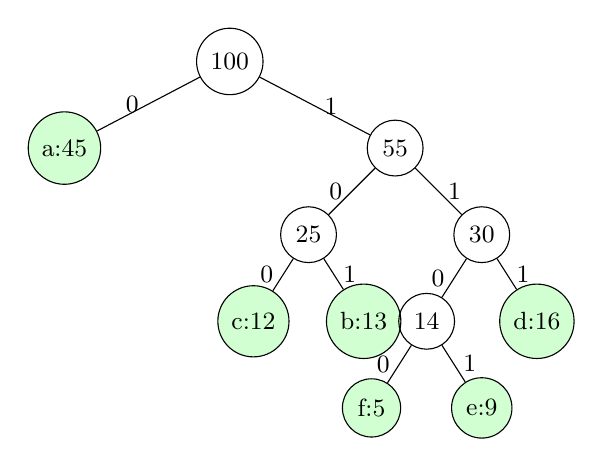
\begin{tikzpicture}[level distance=11mm,
  level 1/.style={sibling distance=42mm},
  level 2/.style={sibling distance=22mm},
  level 3/.style={sibling distance=14mm},
  every node/.style={font=\small}]
  \node[circle,draw] {100}
    child {node[circle,draw,fill=green!18] {a:45} edge from parent node[left]{0}}
    child {node[circle,draw] {55}
      child {node[circle,draw] {25}
        child {node[circle,draw,fill=green!18] {c:12} edge from parent node[left]{0}}
        child {node[circle,draw,fill=green!18] {b:13} edge from parent node[right]{1}}
        edge from parent node[left]{0}}
      child {node[circle,draw] {30}
        child {node[circle,draw] {14}
          child {node[circle,draw,fill=green!18] {f:5} edge from parent node[left]{0}}
          child {node[circle,draw,fill=green!18] {e:9} edge from parent node[right]{1}}
          edge from parent node[left]{0}}
        child {node[circle,draw,fill=green!18] {d:16} edge from parent node[right]{1}}
        edge from parent node[right]{1}}
      edge from parent node[right]{1}};
\end{tikzpicture}
\caption{The optimal Huffman tree for the six-character file. Internal nodes show
the combined frequency of their subtree; leaves (green) show character and
frequency. Codewords: $a=\texttt{0}$, $c=\texttt{100}$, $b=\texttt{101}$,
$f=\texttt{1100}$, $e=\texttt{1101}$, $d=\texttt{111}$.}
\label{ch16:huffman-tree}
\end{figure}

The number of bits to encode the whole file is the sum, over all characters $x$,
of (frequency of $x$) $\times$ (depth of $x$'s leaf), because the depth is
exactly the codeword length. Define the cost of a tree $T$ as
\[
  B(T) = \sum_{x} f(x)\, d_T(x),
\]
where $f(x)$ is the frequency and $d_T(x)$ is the leaf depth. Minimizing $B(T)$
over all prefix-free codes is precisely the compression problem. For the tree in
Figure~\ref{ch16:huffman-tree}:
\[
  B = 45(1) + 13(3) + 12(3) + 16(3) + 9(4) + 5(4)
    = 45 + 39 + 36 + 48 + 36 + 20 = 224.
\]
So this code uses $224{,}000$ bits versus the fixed code's $300{,}000$ -- a
$25\%$ saving, achieved simply by assigning $a$ one bit and giving $f$ four.

\subsection{Huffman's greedy idea}

How do we \emph{find} the cheapest tree? Huffman's insight, from a 1951 term
paper, is to build the tree greedily \emph{bottom-up}. The two rarest
characters should sit deepest in the tree (longest codewords), so \emph{merge
them first}: make them siblings under a new internal node whose frequency is the
sum of theirs. Now treat that merged node as a single ``character'' with the
combined frequency, and repeat. Each step fuses the two lowest-frequency items
into one, until a single tree remains.

\begin{intuitionbox}
Think of it as a tournament run in reverse. The two \emph{weakest} (rarest)
players are knocked out first -- buried deepest in the bracket -- by being paired
off and replaced by a team carrying their combined weight. You keep pairing the
two weakest survivors. The last team standing is the root, and the depth at which
a character was eliminated is the length of its codeword. Rare characters get
eliminated early (deep), frequent ones survive late (shallow), which is what
you want.
\end{intuitionbox}

The natural data structure for ``repeatedly extract the two smallest'' is a
\emph{min-priority queue} (a min-heap, from Chapter~6). Here is the algorithm.

\begin{algorithm}[H]
\caption{\textsc{Huffman}($C$)}
\KwIn{A set $C$ of $n$ characters, each with a frequency $f(c)$.}
\KwOut{The root of an optimal prefix-free coding tree.}
$n \leftarrow |C|$\;
$Q \leftarrow$ a min-priority queue on $C$, keyed by frequency\;
\For{$i \leftarrow 1$ \KwTo $n-1$}{
  allocate a new node $z$\;
  $x \leftarrow \textsc{Extract-Min}(Q)$ \tcp*{rarest remaining}
  $y \leftarrow \textsc{Extract-Min}(Q)$ \tcp*{second rarest}
  $z.\mathit{left} \leftarrow x$;\quad $z.\mathit{right} \leftarrow y$\;
  $f(z) \leftarrow f(x) + f(y)$\;
  $\textsc{Insert}(Q, z)$ \tcp*{the merged node rejoins the pool}
}
\Return $\textsc{Extract-Min}(Q)$ \tcp*{the one node left is the root}
\end{algorithm}

\subsection{A full build, traced}

Run \textsc{Huffman} on our six characters by hand. Start with the queue
holding all six, sorted by frequency:
\[
  Q = [\,f{:}5,\ e{:}9,\ c{:}12,\ b{:}13,\ d{:}16,\ a{:}45\,].
\]

\textbf{Step 1.} Extract the two smallest: $f{:}5$ and $e{:}9$. Merge them under a
new node $z_1$ with frequency $5+9 = 14$. Reinsert:
\[
  Q = [\,c{:}12,\ b{:}13,\ z_1{:}14,\ d{:}16,\ a{:}45\,].
\]

\textbf{Step 2.} Extract $c{:}12$ and $b{:}13$. Merge under $z_2$ with frequency
$25$. Reinsert:
\[
  Q = [\,z_1{:}14,\ d{:}16,\ z_2{:}25,\ a{:}45\,].
\]

\textbf{Step 3.} Extract $z_1{:}14$ and $d{:}16$. Merge under $z_3$ with frequency
$30$. Reinsert:
\[
  Q = [\,z_2{:}25,\ z_3{:}30,\ a{:}45\,].
\]

\textbf{Step 4.} Extract $z_2{:}25$ and $z_3{:}30$. Merge under $z_4$ with
frequency $55$. Reinsert:
\[
  Q = [\,a{:}45,\ z_4{:}55\,].
\]

\textbf{Step 5.} Extract $a{:}45$ and $z_4{:}55$. Merge under $z_5$ with frequency
$100$. This is the root.
\[
  Q = [\,z_5{:}100\,].
\]

Five merges for six leaves -- exactly the $n-1 = 5$ iterations the loop predicts.
And the tree we just built, with $z_5$ as root, $a$ hanging off it at depth $1$,
and $f,e$ buried at depth $4$, is \emph{precisely}
Figure~\ref{ch16:huffman-tree}. The greedy ``merge the two rarest'' rule
reconstructed the optimal code without ever comparing it to an alternative.

Figure~\ref{ch16:huffman-merges} lays the five steps out as a queue that shrinks
by one item per merge: read each row left to right, watch the two smallest keys
disappear and their sum reappear, until a single root key of $100$ remains.

\begin{figure}[h]
\centering
\begin{tikzpicture}[font=\scriptsize, node distance=2mm,
  itm/.style={draw, rounded corners=1pt, minimum height=5mm, inner sep=2pt},
  picked/.style={itm, fill=trapred!18},
  made/.style={itm, fill=targetgreen!20}]
  \def\rowsep{6.5mm}
  % step labels and rows
  \foreach \lbl/\y in {start/0, after 1/1, after 2/2, after 3/3, after 4/4, after 5/5}
    \node[anchor=east, font=\scriptsize\itshape] at (-0.4, -\y*\rowsep) {\lbl};
  % each row is a queue state; the two red nodes are extracted next to form the
  % node that appears in the following row.
  % row 0 (start)
  \node[picked] (r0a) at (0,0) {$f{:}5$};
  \node[picked, right=of r0a] (r0b) {$e{:}9$};
  \node[itm, right=of r0b] (r0c) {$c{:}12$};
  \node[itm, right=of r0c] (r0d) {$b{:}13$};
  \node[itm, right=of r0d] (r0e) {$d{:}16$};
  \node[itm, right=of r0e] (r0f) {$a{:}45$};
  % row 1
  \node[picked] (r1a) at (0,-\rowsep) {$c{:}12$};
  \node[picked, right=of r1a] (r1b) {$b{:}13$};
  \node[itm, right=of r1b] (r1c) {$z_1{:}14$};
  \node[itm, right=of r1c] (r1d) {$d{:}16$};
  \node[itm, right=of r1d] (r1e) {$a{:}45$};
  % row 2
  \node[picked] (r2a) at (0,-2*\rowsep) {$z_1{:}14$};
  \node[picked, right=of r2a] (r2b) {$d{:}16$};
  \node[itm, right=of r2b] (r2c) {$z_2{:}25$};
  \node[itm, right=of r2c] (r2d) {$a{:}45$};
  % row 3
  \node[picked] (r3a) at (0,-3*\rowsep) {$z_2{:}25$};
  \node[picked, right=of r3a] (r3b) {$z_3{:}30$};
  \node[itm, right=of r3b] (r3c) {$a{:}45$};
  % row 4
  \node[picked] (r4a) at (0,-4*\rowsep) {$a{:}45$};
  \node[picked, right=of r4a] (r4b) {$z_4{:}55$};
  % row 5: the root
  \node[made] (r5a) at (0,-5*\rowsep) {$z_5{:}100$};
\end{tikzpicture}
\caption{The priority queue across the five Huffman merges, one row per state.
In each row the two red nodes are the smallest keys; they are extracted and
merged, and their sum appears in the next row in sorted position (e.g.\ $f{:}5$
and $e{:}9$ become $z_1{:}14$). The queue shrinks by one each step until only the
root $z_5{:}100$ (green) remains.}
\label{ch16:huffman-merges}
\end{figure}

\begin{labbox}
Re-trace the build but keep a running list of codewords. After step 1, $f$ and
$e$ each have a tentative last bit ($f=\texttt{0\ldots}$, $e=\texttt{1\ldots}$);
every later merge \emph{prepends} a bit to everything in the merged subtree.
Watch $a$ stay a lone leaf until the very last merge, earning it the single bit
\texttt{0}. This ``prepend on merge'' view is why the rarest characters
accumulate the most bits.
\end{labbox}

\subsection{Complexity}

The loop runs $n-1$ times. Each iteration does two \textsc{Extract-Min}s and one
\textsc{Insert} on a heap of size at most $n$, and each heap operation costs
$O(\log n)$. Building the initial heap costs $O(n)$. So the recurrence is just a
sum:
\[
  T(n) = \underbrace{O(n)}_{\text{build heap}} + (n-1)\cdot \underbrace{O(\log n)}_{\text{per merge}} = O(n \log n).
\]

\begin{complexitybox}
\textsc{Huffman} runs in $O(n \log n)$ time using a binary min-heap, where $n$ is
the number of distinct characters. With a more clever structure (keeping the
input pre-sorted and using two queues), it can be done in $O(n \log n)$ for the
sort plus $O(n)$ for the merging -- but the heap version is the one to remember.
The output tree has $n$ leaves and $n-1$ internal nodes, so it uses $O(n)$ space.
\end{complexitybox}

\subsection{Why Huffman is optimal}

We must prove that greed is optimal here too. The proof rests on two lemmas, both
using the same kind of exchange argument that worked for activity selection.

\begin{lemma}[The greedy choice is safe]
\label{ch16:huffman-lemma1}
Let $x$ and $y$ be the two characters with lowest frequency. Then there is an
optimal prefix-free code in which $x$ and $y$ have codewords of the same length
that differ only in the last bit -- that is, $x$ and $y$ are sibling leaves at
the \emph{maximum depth} of the tree.
\end{lemma}

\begin{formalbox}
\textbf{Proof sketch.} Take any optimal tree $T$. Let $b$ and $c$ be two sibling
leaves at maximum depth (a deepest internal node has two leaf children -- it must,
or the tree could be improved). Without loss of generality $f(b) \le f(c)$, and
since $x, y$ are the two least frequent overall, $f(x) \le f(b)$ and
$f(y) \le f(c)$.

Now \emph{swap} $x$ with $b$ to form $T'$, then swap $y$ with $c$ to form $T''$
(if $x$ already happens to be $c$, then $f(x) \le f(b) \le f(c) = f(x)$ forces
$f(b) = f(c)$, so relabel siblings $b$ and $c$ first so $x = b$).
The change in cost from the first swap is
\[
  B(T) - B(T') = \bigl(f(b) - f(x)\bigr)\bigl(d_T(b) - d_T(x)\bigr) \ge 0,
\]
because $f(b) \ge f(x)$ (the swapped-in character is rarer) and $d_T(b) \ge
d_T(x)$ ($b$ was at maximum depth). So the swap does not \emph{increase} cost.
The same holds for the second swap. Hence $B(T'') \le B(T)$, but $T$ was optimal,
so $B(T'') = B(T)$ and $T''$ is also optimal -- and in it, $x$ and $y$ are
deepest siblings. $\qquad\blacksquare$
\end{formalbox}

The intuition behind that inequality drives the whole algorithm:
\emph{putting a rarer character deeper never costs more.} If a frequent character
sits deep and a rare one sits shallow, swapping them can only help, because you
pay the deep (long) codeword on fewer occurrences. The least frequent characters
\emph{belong} at the bottom.

\begin{lemma}[Optimal substructure]
\label{ch16:huffman-lemma2}
Let $z$ be the merged node replacing siblings $x$ and $y$, with $f(z) = f(x) +
f(y)$. If $T'$ is an optimal tree for the reduced alphabet (with $z$ in place of
$x,y$), then the tree $T$ obtained from $T'$ by re-splitting $z$ into its
children $x$ and $y$ is optimal for the original alphabet.
\end{lemma}

\begin{formalbox}
\textbf{Proof idea.} The two trees' costs differ by a fixed, choice-independent
amount. When we split $z$ at depth $d$ into $x$ and $y$ at depth $d+1$, the cost
changes by
\[
  B(T) - B(T') = \bigl(f(x) + f(y)\bigr)(d{+}1) - \bigl(f(x)+f(y)\bigr)d = f(x)+f(y),
\]
a constant. So minimizing $B(T')$ is the same as minimizing $B(T)$: an optimal
reduced tree gives an optimal full tree. Combining this with
Lemma~\ref{ch16:huffman-lemma1} (the merge was a safe choice) and inducting on
the alphabet size proves \textsc{Huffman} optimal. $\qquad\blacksquare$
\end{formalbox}

\begin{historybox}
David Huffman invented optimal prefix coding in 1951 as a graduate student at MIT. His professor, Robert Fano, offered students a choice between a final exam and a term paper on finding the most efficient binary prefix-free code for known symbol frequencies. Claude Shannon and Fano had proposed a top-down probability-splitting heuristic (Shannon--Fano coding), yet it sometimes missed the true optimum.

After weeks of dead ends, Huffman was ready to toss his notes and study for the exam when the key inversion struck him: instead of splitting top-down, merge bottom-up from the two rarest symbols. Two decades later, Jack Edmonds (1971) connected greedy algorithms to matroid theory (introduced by Hassler Whitney in 1935), proving that for hereditary set systems, the heaviest-first greedy algorithm is optimal for \emph{every} nonnegative weight function if and only if the independent sets satisfy the matroid exchange axiom.

Because greedy algorithms look deceptively simple when they work (fractional knapsack, minimum spanning trees, Huffman coding), a classic trap is trusting an unproved greedy rule on a neighbor problem where it fails --- such as 0-1 knapsack or weighted interval scheduling. Small constraint changes (arbitrary task lengths, capacities, or intersecting two matroids) routinely break the greedy-choice property and force a return to dynamic programming or approximation algorithms.
\end{historybox}

\section{Why does greed work? A glimpse of matroids}

You now have two greedy success stories and one greedy failure (the $\{1,3,4\}$
coins). It would be wonderful to have a \emph{single} theorem that says, ``If your
problem has this abstract shape, greed is guaranteed optimal -- proof not
required.'' Such a theorem exists for a large family of problems. The
abstraction is called a \emph{matroid}, and it is a central idea in
combinatorics.

\subsection{The pattern behind the proofs}

Look back at activity selection and Huffman. Both proofs had the same two moving
parts: a notion of a partial solution you can \emph{extend} (a compatible set you
can add to; a tree you can keep merging), and an \emph{exchange} step (swap the
greedy choice in without loss). A matroid is an abstract structure that
guarantees both parts work.

\begin{definition}[Matroid]
\label{ch16:def-matroid}
A \emph{matroid} is a pair $M = (S, \mathcal{I})$ where $S$ is a finite set and
$\mathcal{I}$ is a collection of subsets of $S$ -- the \emph{independent} sets --
satisfying:
\begin{enumerate}
\item \textbf{(Nonempty)} $\emptyset \in \mathcal{I}$.
\item \textbf{(Hereditary)} If $A \in \mathcal{I}$ and $B \subseteq A$, then
  $B \in \mathcal{I}$. Every subset of an independent set is independent.
\item \textbf{(Exchange)} If $A, B \in \mathcal{I}$ and $|A| < |B|$, then there is
  some element $x \in B \setminus A$ such that $A \cup \{x\} \in \mathcal{I}$.
  A smaller independent set can always be grown using an element from any larger
  one.
\end{enumerate}
\end{definition}

The word ``independent'' is borrowed from linear algebra, and that is the
canonical example: let $S$ be a set of vectors and let $\mathcal{I}$ be the
collection of \emph{linearly independent} subsets. Property 2 holds (a subset of
independent vectors is independent), and property 3 is a classic fact of linear
algebra (a smaller independent set can be extended toward any basis). That is
where the whole vocabulary -- ``independent,'' ``rank,'' ``basis'' -- comes from.

\begin{intuitionbox}
Informally, a matroid is a setting where ``a valid
partial solution'' (an independent set) has two friendly properties: you can
always shrink it and stay valid (hereditary), and if your partial solution is
smaller than someone else's, you can always borrow one of their elements to grow
yours (exchange). Those are exactly the two things an exchange-argument
correctness proof needs, so checking the axioms once gives you the proof.
\end{intuitionbox}

\subsection{The greedy theorem for matroids}

In a \emph{weighted} matroid, each element $x \in S$ carries a positive weight
$w(x)$, and we want a \emph{maximum-weight} independent set. The greedy algorithm
is the obvious one: sort elements by weight, heaviest first, and add each to your
set if it keeps the set independent.

\begin{algorithm}[H]
\caption{\textsc{Greedy}($M, w$)}
\KwIn{A matroid $M = (S, \mathcal{I})$ and a weight function $w$.}
\KwOut{A maximum-weight independent set $A$.}
$A \leftarrow \emptyset$\;
sort $S$ into nonincreasing order by weight $w$\;
\For{each $x \in S$ taken in that order}{
  \If{$A \cup \{x\} \in \mathcal{I}$}{
    $A \leftarrow A \cup \{x\}$\;
  }
}
\Return $A$
\end{algorithm}

\begin{theorem}[Greedy is optimal on any matroid]
\label{ch16:thm-matroid}
If $M = (S, \mathcal{I})$ is a matroid with positive weights $w$, then
\textsc{Greedy}$(M, w)$ returns a maximum-weight independent set.
\end{theorem}

Why does this hold? Let $x$ be the first (heaviest) element of $S$ such that
$\{x\} \in \mathcal{I}$. If an optimal independent set $B$ does not already
contain $x$, grow $A = \{x\}$ by repeatedly applying the exchange axiom against
$B$ until $|A| = |B|$: every element of $A \setminus \{x\}$ comes from $B$, so
$A = (B \setminus \{y\}) \cup \{x\}$ for some $y \in B$ with $w(y) \le w(x)$,
making $A$ at least as heavy as $B$ (greedy-choice property). Restricting $M$ to
elements remaining compatible with $x$ yields a smaller matroid, and induction
finishes the proof.

Notice what this theorem \emph{buys} you. Minimum spanning trees (Chapter~23's
Kruskal algorithm is greedy on the \emph{graphic matroid} of a graph, with edge
weights inverted), unit-time task scheduling with deadlines and penalties, and
selecting maximum-weight linearly independent vector bases are all
\emph{instances} of weighted matroids. For each, you do not need to invent a new
exchange argument: you check the three matroid axioms once, and
Theorem~\ref{ch16:thm-matroid} hands you optimality for free.

\begin{aestheticbox}
This is the payoff of abstraction. The first time you prove a greedy algorithm
correct, it feels like a clever, problem-specific trick. The matroid theorem
shows that it is an instance of a general structural result. When
you later meet Kruskal's minimum-spanning-tree algorithm and someone says ``it's
just greedy on the graphic matroid,'' you will understand both \emph{why} it is
correct and why you do not have to re-derive its proof from scratch. Good
abstractions turn many proofs into one.
\end{aestheticbox}

\begin{remark}
Not every greedy success is a matroid. Compatible intervals in activity
selection, for instance, violate the exchange axiom: a single long interval
$A = \{[0,10)\}$ is smaller than $B = \{[1,4), [5,9)\}$, yet neither interval of
$B$ can be added to $A$ without overlapping (which is why \emph{weighted}
activity selection needs dynamic programming, while unweighted activity selection
needed our finish-time exchange proof). Likewise, Huffman coding is not a
weighted matroid and genuinely needs the two lemmas we proved. Matroids capture a
\emph{large} class of greedy-friendly problems --- precisely the hereditary ones
where heaviest-first greed works for \emph{every} weight function --- while
broader frameworks (matroid intersection, greedoids, and submodular optimization)
push further beyond this book.
\end{remark}

\begin{walkbox}
Here is a matroid to verify on your walk. Let $S$ be the edges of a connected
graph, and let $\mathcal{I}$ be all subsets of edges that contain \emph{no cycle}
(the ``forests''). Convince yourself the hereditary property holds -- remove an
edge from a forest and it is still a forest. The exchange property is subtler:
if forest $A$ has fewer edges than forest $B$, why must some edge of $B$ extend
$A$ without making a cycle? Sketch a small graph and feel it out. You will have
discovered the \emph{graphic matroid}, the structure that makes Kruskal's
algorithm correct when we study minimum spanning trees in Chapter~23.
\end{walkbox}

\section{Summary}

Greed is the strategy of committing to the locally best choice and never looking
back. It is much faster and simpler than dynamic programming \emph{when
it works} -- and it works exactly when a problem has the greedy-choice property
on top of optimal substructure. The recurring proof technique is the
\emph{exchange argument}: show any optimal solution can be edited to contain the
greedy choice without getting worse.

We saw greed succeed for activity selection (earliest finish wins, $\Theta(n)$
after sorting) and for Huffman coding (merge the two rarest, $O(n \log n)$), and
we saw it fail for coin change under the $\{1,3,4\}$ system, where dynamic
programming was required. Finally, matroids gave us a glimpse of \emph{why} greed
works at all: for a whole family of problems, three abstract axioms guarantee
optimality, turning many separate exchange proofs into a single theorem you can
reuse. Keep that lens in mind; we will see the graphic matroid in action when we study minimum
spanning trees in Chapter~23.

Greedy algorithms and dynamic programming both tackle optimization problems by
exploiting optimal substructure. But whether we commit greedily or evaluate
subproblems across a table, we have so far measured the cost of an algorithm by its
worst-case performance on a single operation.

In many real systems, however, individual operations vary wildly. A dynamic array
might append in $O(1)$ time for a thousand steps, then suddenly freeze for an $O(n)$
resizing pass before returning to $O(1)$ appends. Calling every append $O(n)$ because
of that rare spike is overly pessimistic: over any sequence of $n$ operations, the
total work is only $O(n)$, averaging $O(1)$ per operation. In \textbf{Chapter~17
(Amortized Analysis)}, we develop three formal methods -- the aggregate method, the
accounting method, and the potential method -- to analyze operations that are
individually erratic but collectively cheap.

\section*{Exercises}
\addcontentsline{toc}{section}{Exercises}

\begin{exercise}
Run \textsc{Greedy-Activity-Selector} by hand on the activities (given as
$(s,f)$ pairs) $(1,3)$, $(2,5)$, $(4,7)$, $(1,8)$, $(5,9)$, $(8,10)$, $(9,11)$.
List the chosen set and its size. (Remember to sort by finish time first.)
\end{exercise}

\begin{exercise}
Give a concrete counterexample showing that the ``pick the activity with the
earliest \emph{start} time'' greedy rule can be suboptimal. Three activities are
enough.
\end{exercise}

\begin{exercise}
For U.S. coins $\{1, 5, 10, 25\}$, prove that the greedy ``largest coin first''
rule is optimal for making any amount $n$. (Hint: argue about how many of each
smaller coin an optimal solution can contain before it would be cheaper to use a
larger one.)
\end{exercise}

\begin{exercise}
Find the smallest amount $n$ for which greedy coin change fails under the system
$\{1, 4, 6\}$, and exhibit both the greedy answer and a strictly better one.
\end{exercise}

\begin{exercise}
Build the Huffman tree for the frequencies $a{:}10$, $b{:}15$, $c{:}30$,
$d{:}16$, $e{:}29$. Show the priority queue after each merge, draw the final
tree, and compute the total encoded length $B(T)$.
\end{exercise}

\begin{exercise}
Suppose all $n$ characters have \emph{equal} frequency. What shape does the
Huffman tree take, and what are the codeword lengths? Relate your answer to the
fixed-length code. (Consider separately the cases where $n$ is and is not a power
of two.)
\end{exercise}

\begin{exercise}
Prove that in any optimal prefix-free code, the character with the highest
frequency has a codeword of length $1$ \emph{or} shares the minimum codeword
length with at least one other character. (Hint: exchange argument, mirroring
Lemma~\ref{ch16:huffman-lemma1}.)
\end{exercise}

\begin{exercise}
A Huffman tree is built greedily; suppose instead you (wrongly) always merge the
two \emph{most} frequent items. On the six-character file of this chapter, build
that tree and compute its cost. By how many bits does it lose to the optimal
$224{,}000$?
\end{exercise}

\begin{exercise}[Matroid check]
Let $S$ be a finite set and let $\mathcal{I}$ consist of all subsets of $S$ of
size at most $k$, for a fixed integer $k$. Verify that $(S, \mathcal{I})$
satisfies the three matroid axioms. (This is the \emph{uniform matroid}; greedy
on it just picks the $k$ heaviest elements.)
\end{exercise}

\begin{exercise}[Challenge]
You have $n$ tasks; task $i$ takes time $t_i$ on a single machine. If you run them
in some order, the \emph{completion time} of a task is when it finishes, and you
want to minimize the \emph{sum} of all completion times. Propose a greedy rule,
and prove it optimal with an exchange argument. (Hint: think about which task you
would never want to schedule last.)
\end{exercise}

\begin{exercise}[Challenge]
Prove the optimal-substructure direction for activity selection rigorously: if
$A_{ij}$ denotes a maximum-size compatible set drawn entirely from the activities
that start after $a_i$ finishes and finish before $a_j$ starts, and if $a_k \in
A_{ij}$, show that $A_{ij} = A_{ik} \cup \{a_k\} \cup A_{kj}$ where $A_{ik}$ and
$A_{kj}$ are themselves optimal for their sub-ranges. Use a cut-and-paste
argument.
\end{exercise}
